\documentclass{beamer}
\usepackage[english,french]{layout}
\usepackage[utf8]{inputenc}
\usepackage[english]{babel}
\usepackage[T1]{fontenc}
\usepackage{lmodern}
\usepackage{textcomp}
\usepackage{amsmath, soul, color, multicol, type1cm, verbatim, latexsym, dsfont, float, listings,alltt}
\usepackage[official]{eurosym}
\usepackage{beamerthemesplit}
\usetheme{Frankfurt}
\usefonttheme{professionalfonts}
\setbeamercovered{transparent}
%NeSI Colors <-------------------------------------------------------------------------------------
\usecolortheme{lily}
\usecolortheme[RGB={47, 68, 71}]{structure} 
\definecolor{nesidark}{HTML}{2F4447}
\definecolor{nesilight}{HTML}{CED9DF}
\definecolor{nesigrey}{gray}{0.7}
\definecolor{nesilightgrey}{gray}{0.98}
\definecolor{nesidarkgrey}{gray}{0.3}
\definecolor{nesiblue}{HTML}{2B9FC2}
\setbeamercolor{block title}{fg=black,bg=nesigrey}
\setbeamercolor{block body}{bg=nesilightgrey,fg=nesidarkgrey}
\setbeamercolor{block body alerted}{bg=white,fg=black}
\setbeamercolor{alerted text}{bg=white,fg=black}
%NeSI Title <---------------------------------------------------------------------------------------
\setbeamerfont{title}{size=\huge}
\frenchspacing
\hyphenation{NeSI}
%NeSI Template parameters <-------------------------------------------------------------------------
\setbeamertemplate{blocks}[default]
\useinnertheme{circles}
\setbeamertemplate{title page}[default][center,rounded=false,shadow=false]
\newcommand\BackgroundPicture[1]{%
\setbeamertemplate{background}{%
\parbox[c][\paperheight]{\paperwidth}{%
\vfill \hfill \includegraphics[height=0.9\paperheight]{#1}
\hfill \vfill
}}}

%Content Starts Here <-------------------------------------------------------------------------------
\title{Rapid Parameterisation of Small Molecules}
%\subtitle{Computational Science team}
\author{Dr Benjamin Roberts \\ (ben.roberts@nesi.org.nz)}
\date{23 March 2015}

\begin{document}

{
\setbeamertemplate{background canvas}{
\includegraphics[height=0.99\paperheight]{NeSI_img/Slide00.png}} 
\begin{frame}[plain]
\vspace{1cm}
\titlepage
\end{frame}
}


% This will generate the outline. If you have several topics, uncomment the multicols 
\begin{frame}
\frametitle{Outline}
% \begin{multicols}{2} 
   \tableofcontents
% \end{multicols}
\end{frame}


%%%%%%%%%%%%%%%%%%%%%%%%%%%%%%%%%%%%%%%%%%%%%%%%%%%%%%%%%%%%%%%%%%%%%%%%%%%%%%%%%%%%%%%%%%%%%%%
%%%%%%%%%%%%%%%%%%%%%%%%%%%%%%%%%%%%%%%% Some Examples %%%%%%%%%%%%%%%%%%%%%%%%%%%%%%%%%%%%%%%%%%%
%%%%%%%%%%%%%%%%%%%%%%%%%%%%%%%%%%%%%%%%%%%%%%%%%%%%%%%%%%%%%%%%%%%%%%%%%%%%%%%%%%%%%%%%%%%%%%%

\section{Introduction}

\frame[t]
{
\frametitle{Molecular Mechanics}
\begin{itemize}
\item An approximation of a molecule's potential energy using a Newtonian model
\item Add a time component to get molecular dynamics (MD)
\item The system is represented in three parts: Coordinates, topology and force field
\item Coordinates: Where all the particles are (arbitrary frame of reference)
\item Topology: Which particles are connected to which other particles
\item What is a force field?
\end{itemize}
}

\frame[t]
{
\frametitle{Force fields}
\begin{center}
{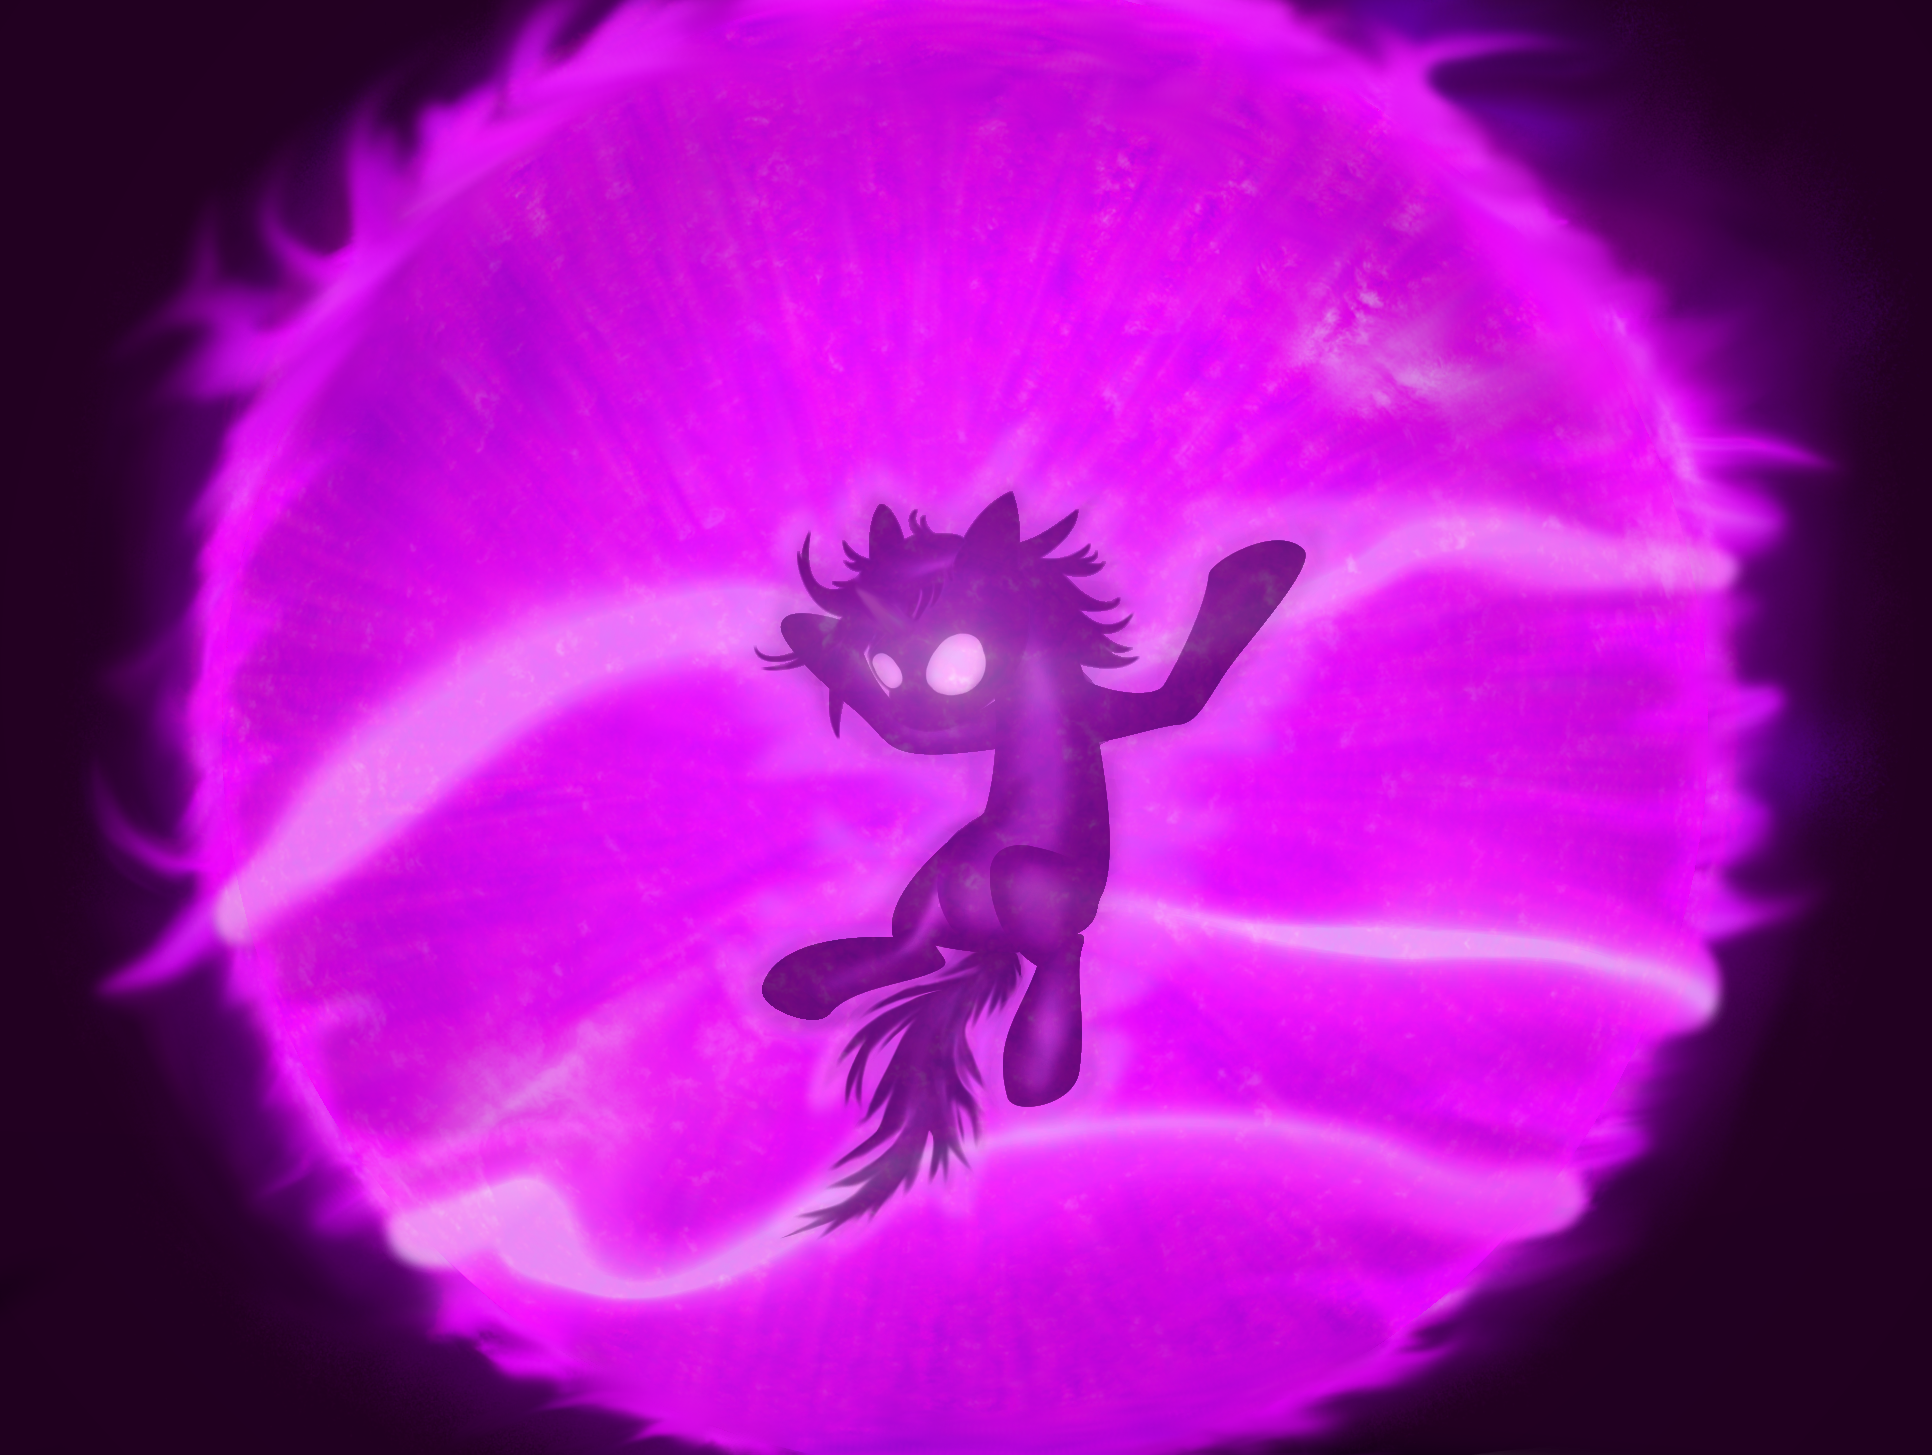
\includegraphics[height=0.45\paperheight]{force_field_by_konsumo-d78g7nt.png}}
\end{center}
A force field is an approximate mathematical model of the potential energy surface of the system.
It can be expressed as an equation in \(3N - 6\) variables, where \(N\) is the number of particles.
}

\frame[t]
{
\frametitle{Force fields}
\begin{block}{Functional form}
	\begin{itemize}
		\item The form of the equations used to model the various types of interaction that contribute to the overall potential energy (bond stretching, angle bending, etc.)
		\item All interactions of the same class will use the same basic model (e.g., bonds commonly use a quadratic equation in the manner of Hooke's law)
	\end{itemize}
\end{block}
\begin{block}{Parameters}
	\begin{itemize}
		\item The constant terms used in the equations
		\item Within any given class, each specific type of interaction will have its own parameters
		\item Individual interaction types are often quite fine-grained
	\end{itemize}
\end{block}
}


\section{Technical Overview}
\frame[t]
{
\frametitle{Technical Overview}
 There are three structured approaches to run our jobs on a MPI machine
\begin{enumerate}
 \item MPMD
 \item batcher
 \item custom (usually a form of the previous two but integrated within your workflow)
\end{enumerate}
We will use three case studies to show the problems and the solutions adopted.
}

\section{Case Studies}

\subsection{presentation}
\frame[t]{
\frametitle{Case Studies}
\begin{block}{Presentation}
We'll go through the work of three researchers showing various problems and solutions and we'll summarize their pros and cons.
\begin{enumerate}
 \item Ehsan's simulations (the flood)
 \item Nick's network (MPMD in testing)
 \item Jing Wang: DNA matching (batcher)
\end{enumerate}
\end{block}
}
\subsection{Eshan's Simulations}
\frame[t]{
\frametitle{Ehsan's Simulations}
Ehsan is a PhD student in computer science. His problem is simulating wireless networks to improve the efficiency of the communication in mobile devices.

\begin{itemize}
\item first submission to the cluster was 40,000 simulations
\item done 4 at a time
\item first reaction: increase the number of simulations he can run (after all they are not big MPI jobs)
\item Bad idea: the simulations were spread all over the cluster blocking big MPI jobs
\item developed a custom solution to contain him to a set of nodes
\item we later found out that it was equivalent to using MPMD
\end{itemize}
We now identify high-throughput project quickly and offer them better solutions as soon as possible.
}

\subsection{Nick's networks}
\frame[t]{
\frametitle{Nick's Networks}
\begin{itemize}
\item Nick Baker is a PhD student in biological sciences with a background in mathematics. He studies ecological networks (complex food chains).

\item His work focuses on analysing networks to find "keystone" species that are essential to the network. The work is what we call embarassingly parallel, he has to go through a high number of networks and perfoorm his analyses on each and everyone of them.

\item I spotted him on the cluster running running four jobs at a time out of close to a hundred. There was definitely room for improvement. He became a test subject for MPMD
\end{itemize}
}
\frame[t]{
\frametitle{MPMP: Multiple Program Multiple Data}
\begin{multicols}{2}
\begin{figure}
\end{figure}
SMPD: Instances of a program process the data distributed amongst them.
\begin{figure}
\end{figure}
MPMD: Programs, not necessarily identical, process distinct data.
\end{multicols}
}
{
\setbeamertemplate{background canvas}{
\includegraphics[height=0.99\paperheight]{NeSI_img/Slide00.png}} 
\begin{frame}[plain]
\begin{center}
{\Huge Questions \& Answers}
\end{center}
\end{frame}
}


\end{document} 
